\documentclass[12pt]{turabian-researchpaper}
\usepackage{graphicx}
\usepackage{amsmath}
\usepackage{amsfonts}
\usepackage{float}
\usepackage{xcolor}
\usepackage[pass, letterpaper]{geometry}
\DeclareMathOperator*{\argmax}{arg\,max}
%\usepackage[notes,backend=biber]{biblatex-chicago}
%\usepackage[authordate,backend=biber]{biblatex-chicago}
%\usepackage[authordate-trad,backend=biber]{biblatex-chicago}
\usepackage[authordate,backend=biber]{biblatex-chicago}

\addbibresource{464_final.bib}

\providecommand{\keywords}[1]{\textbf{\textit{Keywords:}} #1}

\title{Chess Reinforcement Methods}
\subtitle{Using Reinforcement Agents to Play Chess}
\author{Ethan Colen, Brian Elinsky, Chris Festa, Philmore Morrison}
%\submissioninfo{Supporting repo: https://github.com/hellion87/MSDS_464_FINAL.git}
\date{December 10, 2021}
\begin{document}
\maketitle

\begin{abstract}
    \noindent
    Chess is one of the most studied domains of artificial intelligence. Unfortunately, the massive branching factor and state-space make an exhaustive search intractable. We introduce multiple methods to build a chess-playing algorithm to overcome these challenges. First, we evaluate a Monte Carlo Search Tree (MCST) agent that uses an Upper Confidence Bounds for Trees (UCT) algorithm for the tree policy and acts randomly for the rollout policy. This algorithm performs poorly when iterating 50,000 times per move, making short-sighted moves because of the shallow search tree. Second, we implement an actor-critic model that uses convolutional networks to generalize by training the agent with 1000 games of self-play. This agent plays better but is still poor. Last, we expand the AlphaGo Zero algorithm by implementing an alternative training target that incorporates temporal difference learning ideas. In our approach, we compute the Q value of each state through repeated simulations from that node. In contrast, the standard AlphaGo Zero algorithm back-propagates the episode reward to estimate the value of state/action pairs. This agent performs best, beating our AlphaGo Zero agent 31 games, losing 19 games, and drawing 50 games. \\
\noindent\keywords{Chess, Stockfish, Policy Estimation, Deep Learning}
\end{abstract}

\section*{Introduction}

%In 1951, Alan Turing was the first to publish a program that could play a full game of chess. The program was crude, and the algorithm could only think two moves in advance. It was not until 1997 when IBM Deep Blue made history when it became the first machine to beat the reigning world chess champion \parencite{goodrich_how_2021}. The Deep Blue system had the ability to evaluate chess moves and was able to search up to 200 million options per second and evaluate multiple lines of attack. 

Chess engines and artificial intelligence has come a long way since Alan Turing’s simple program and IBM Deep Blue. Deep neural networks and reinforcement learning ushered in a new era in creating engines that far surpass Alan Turing’s application and IBM Deep Blue. More recent methods such as AlphaZero combine the latest mainstream reinforcement learning concepts such as Monte Carlo Tree Search, Temporal Difference Learning, and Deep Neural Networks. In reinforcement learning, deep neural networks train approximation functions to represent latent policies and reward functions by learning from experience and rewards. These techniques have learned to play Atari games beyond human-level, Go, chess, and shogi from scratch, among others \parencite{srinivasan_actor-critic_2018}. The purpose of this study is to survey the latest concepts to play chess that makeup Google DeepMind’s AlphaGo and policy-based approaches to reinforcement learning. We explore multiple learning methods for learning policy approximation, and our objective is to train and evaluate different ways to play chess.

%\textbf{ THIS SEEMS BETTER PLACED IN THE LIT REV... -- START}
%The second method, actor-critic, is a training process that is guided by an actor that is a policy function that picks what moves to play and a critic which tracks whether the agent is ahead or behind in the game. The actor-critic method is like a general adversarial network (GAN) where a discriminator and generator play against each other and the generator creates fake images, and the discriminator evaluates how the fake image is compared to the real image \parencite{karunakaran_actor-critic_2020}. The study uses convolutional neural networks (CNN) where the policy approximation function trains over thousands of games.

%The last method, Google DeepMind’s AlphaGo Zero, uses Monte Carlo Tree Search (MCTS) and residual convolutional neural networks (CNN) to create a reinforcement learning agent to play chess. The MCTS chooses its next move by exploring interesting states in a finite time period and the residual CNN assesses the new positions. We implemented an extension of AlphaGo Zero which incorporates temporal difference learning rather than waiting until the end of an episode to update values. This leads to a model which can train faster than predecessor models, including vanilla AlphaGo Zero. Temporal difference methods do not require a model of the environment, its rewards, and the next state probabilities which make temporal difference methods useful in applications where it’s too hard or impractical to understand the environment and future states \parencite{sutton1988learning}. 
%\textbf{ THIS SEEMS BETTER PLACED IN THE LIT REV... -- END}

\section{Literature Review}

A long-standing ambition of artificial intelligence has been to create programs that can instead learn for themselves from first principles \parencite{silver_general_2018}. Researchers have used countless resources in the pursuit of a proficient chess-playing algorithm. Through experience, one might learn to predict whether chess positions will lead to a win \parencite{sutton1988learning}. The game of chess is the longest-studied domain in the history of artificial intelligence \parencite{silver_general_2018}. The seminal works of Claude Shannon, Alan turning, and countless researchers derived the theory and built hardware to play chess efficiently. Chess programs evaluated positions using handcrafted features and carefully tuned weights, constructed by strong human players and programmers, combined with a high-performance alpha-beta search that expands a vast search tree using a large number of clever heuristics and domain-specific adaptations \parencite{silver_general_2018}. Handcrafted heuristics guarantee that subsequent chess algorithms could not be useful outside of the world of chess. There are also too many permutations and moves for humans to hand-code an algorithm effectively. The rules in chess are position and piece dependent. For example, pawns can move two steps forward from the second row (player‘s perspective). The queen can move across the board freely, and under the right circumstances, a player can castle. We can describe a move in chess in two parts. The agent first selects a piece to move, then selects an action from the possible moves for the chosen piece.

Deep Blue was developed at IBM in the 1990s after multiple years of research and development, focusing on building a world-class chess machine \parencite{campbell_deep_2002}. Deep Blue I lost to Garry Kasparov in 1996, four to two. The Deep Blue team modified the Deep Blue architecture and rechallenged Kasparov again in 1997. Deep Blue defeated Garry Kasparov in the 1997 match by a score of 3.5–2.5, and the Deep Blue team was awarded the Fredkin prize for defeating the human world champion in a regulation match \parencite{campbell_deep_2002}. The Deep Blue system could evaluate chess moves and search up to 200 million options per second and evaluate multiple lines of attack. 

Chess subsequently became a grand challenge task for a generation of artificial intelligence researchers, culminating in high-performance computer chess programs that play at a super-human level \parencite{silver_general_2018}. Monte Carlo Tree Search (MCTS) is one such method. MCTS combines Monte Carlo methods and a tree search, a probabilistic algorithm that uses lightweight random simulations to grow a game tree selectively. MCTS is a simple algorithm to implement and can operate with limited domain knowledge \parencite{choudhary_introduction_2019}. The MCTS algorithm consists of the following phases; selection, expansion, simulation, and backpropagation. During the selection phase, the algorithm searches the portion of the tree that has already been represented in memory \parencite{swiechowski2021}. Next, the expansion phase is triggered if the selection phase does not reach a terminal state. The expansion adds nodes corresponding to state s-prime (new-state) based on the previous action. Next, simulation implements the Monte Carlo part of the algorithm to estimate possible reward and terminal state. Finally, backpropagation distributes the simulated scores up the tree to the root node while updating the statistics for visits \(n_i\) and state estimate \(S_i\). 

MCTS has an advantage over traditional depth-limited minimax search by using alpha-beta pruning in games with high branching factors such as Go, minimax search with alpha-beta pruning surpasses MCTS in domains like Chess \parencite{lin_monte_2017}. MCTS does not detect shallow traps as well as minimax search does. Missing a shallow trap can lead to an opponent winning within a few moves.  During minimax search, we build a tree from position \(x\) by examining all possible moves for the computer in that position, then all possible moves for the opponent, followed by all possible moves for the computer to a predetermined depth \(d\) \parencite{baxter_learning_2000}.  

Temporal Difference (TD) learning is another algorithm for learning policies. Arthur Samuel introduced TD learning in 1959. \Textcite{samuel1959} created a checkers playing system based on TD learning. \Textcite{sutton1988learning} contributed to the literature by using TD learning as an incremental learning process for making predictions. TD approximates the expected long-term future cost (or cost-to-go) of a stochastic dynamical system as a function of the current state \parencite{baxter_learning_2000}. The main objective is to minimize the error between the prediction for the current and the next state. TD learning became popular because it combined the advantages of dynamic programming and the Monte Carlo method without the total computational overhead. TD learning also leverages the bootstrap method similar to Dynamic Programming. One significant benefit of TD learning is that we do not need to wait until the end of an episode to compute the \(Q\) value. Said another way, ``TD learning bootstraps like DP, so it does not have to wait till the end of the episode, and like the MC method, it does not require the model dynamics of the environment to compute the value function or the Q function" \parencite{science_understanding_2021}. We provide a visual comparison between MCTS and TD learning in figure \ref{fig:td_mc}. 

\begin{figure}[!ht]
    \centering
    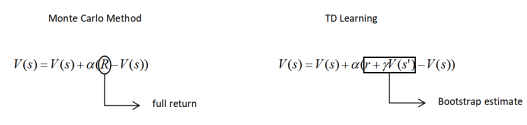
\includegraphics[width=0.95\textwidth]{mcts_td.png}
    \caption{\textit{ Value function based on Monte Carlo tree search versus Temporal Difference learning}}
    \label{fig:td_mc}
\end{figure}

AlphaZero replaces the handcrafted knowledge and domain-specific augmentations used in traditional game-playing programs with deep neural networks, a general-purpose reinforcement learning algorithm, and a general-purpose tree search algorithm \parencite{silver_general_2018}. AlphaZero uses a deep neural network to play chess. The network uses board position as inputs and outputs for move probabilities based on the non-linear evaluations of the board position. AlphaZero learned to approximate the policies through self-play and experience replay based on the Monte Carlo tree search algorithm. AlphaZero can search 60,000 positions per second in chess. \Textcite{silver_general_2018} states that AlphaZero defeated Stockfish when given 1/10 as much thinking time as Stockfish. Stockfish is an open-source chess program ranked as the strongest CPU chess engine in the world. 

Google DeepMind’s AlphaGo Zero uses Monte Carlo Tree Search (MCTS) and residual convolutional neural networks (CNN) to create a reinforcement learning agent to play chess. The MCTS chooses its next move by exploring attractive states in a finite period, and the residual CNN assesses the new positions. We implemented an extension of AlphaGo Zero, which incorporates temporal difference learning rather than waiting until the end of an episode to update values. This leads to a model which can train faster than predecessor models, including vanilla AlphaGo Zero. Furthermore, temporal difference methods do not require a model of the environment, its rewards, and the next state probabilities, making temporal difference methods useful in applications where it’s too hard or impractical to understand the environment and future states \parencite{sutton1988learning}.

Actor-critic methods combine policy and value learning, where researchers use neural networks to approximate an optimal policy.  The policy function plays the actor's role: it picks what moves to play. The value function is the critic: it tracks whether the agent is ahead or behind in the course of the game \parencite{pumperla_chapter_2019}. The feedback loop gets updated during the training process. Actor-critic methods are time-scale algorithms where the critic uses TD learning with a linear approximation architecture; the actor gets updated through gradient estimation based on information provided by the critic. Critic-only methods rely exclusively on value function approximation and aim to learn an approximate solution to the Bellman equation, hopefully prescribing a near-optimal policy \parencite{konda_actor-critic_2000}. The actor decides which action to take, and the critic provides feedback on how good a given action was and how to adjust to optimize the policy. The actor-critic method is like a general adversarial network (GAN) where a discriminator and generator play against each other. The generator creates fake images, and the discriminator evaluates how the fake image is compared to the actual image \parencite{karunakaran_actor-critic_2020}. Since both policy (actor) and value (critic) functions are parametrized and are not guaranteed to converge to optimal values, an agent can quickly converge to some local optimum, which may be far from desired behavior \parencite{ring_replicating_nodate}. One drawback to actor-critic methods is that they suffer from poor sample efficiency. \Textcite{andrychowicz_what_2020} state that a significant obstacle preventing adopting actor-critic methods for control tasks is their poor sample efficiency. Millions of environment interactions are needed to obtain a reasonably performant policy for control problems with moderate complexity. We observe peculiar results in our actor-critic experiment.

We leverage the work of the practitioners that came before us to build three reinforcement learning agents to play chess against the Stockfish chess program. Our agents are based on MCTS, AlphaGo Zero, and an actor-critic agent. First, we discuss various methods and results, followed by a discussion on our findings and future works in the next section.

\section{Methods \& Results}

\subsection{AlphaGo Zero}

To expand upon the AlphaGo Zero algorithm, we implemented an alternative training target that incorporates the ideas of temporal difference learning (TDL). Where the standard AlphaGo Zero algorithm back-propagates the episode reward to estimate the value of state/action pairs, in keeping with Monte Carlo methods, our approach computes the Q value of each state through repeated simulations from that node. In effect, the training target has become the expected result of the game from each position, rather than the actual result \parencite{abrams_lessons_2018}.
We trained two agents for this experiment: one using a standard AlphaGo Zero algorithm, using Monte Carlo tree search, and one using the TDL AlphaGo Zero algorithm. These agents used the same policy network architecture: four convolutional layers with 256 filters, each followed by batch normalization, then two dense layers of 512 nodes, followed by the output layer. After each hidden layer, a rectified linear unit was used as the activation function. Each model was trained purely by self-play for a maximum of 12 GPU-hours. The original AlphaGo Zero model was trained for 64 GPU-days, but we do not have those computational resources available. We hypothesized that the TDL AlphaGo Zero model would train faster than the standard model, so in a fixed amount of time, the TDL model would perform better.

We evaluated our AlphaGo Zero models in two ways: first, by pitting them against the Stockfish chess agent to estimate their Elo ratings, and secondly, by pitting them against each other for 100 games. Using 40 games against Stockfish to estimate Elo, we found the baseline AlphaGo Zero model achieved an Elo rating of 1875, and the TDL AlphaGo Zero achieved an Elo rating of 1949. Against each other, the TDL model won 31 games, the baseline model won 19 games, and 50 games ended in stalemate. 

\subsection{Actor-Critic}
Our actor-critic agent uses multi-layer convolutional neural networks to play chess. We implemented a Q-learning agent for the critic portion of the agent. the agent trained itself for 1000 games before playing against Stockfish. Our actor-critic agent played against Stockfish for 100 games. Even at Stockfish level one, we observed about 50 draws and 25 wins for both Stockfish and our agent. Having 50 ties is quite peculiar when playing against level one Stockfish. 

Based on the preliminary results, we wondered what the actor-critic was learning. The training dataset is significantly imbalanced towards draws. The imbalance is caused by terminating a game after a set number of moves. It is plausible that the actor-critic does now learn to close out games since most of the games end in a draw during training. This assumption led us to add a -0.75 reward for each tie instead of 0, bringing the reward structure to 1 (win), -0.75 (draw), -1 (lose). 

We observed similar results after adjusting the reward structure. The main difference is that we also produced the episodic loss while training the actor-critic. Figure \ref{fig:ac_a_loss} shows a high spike in loss during the earlier episodes, as the agent learns from a shallow replay buffer. Before long, the loss seems to fall, but we see that the loss is increasing over time. 

\begin{figure}[!ht]
    \centering
    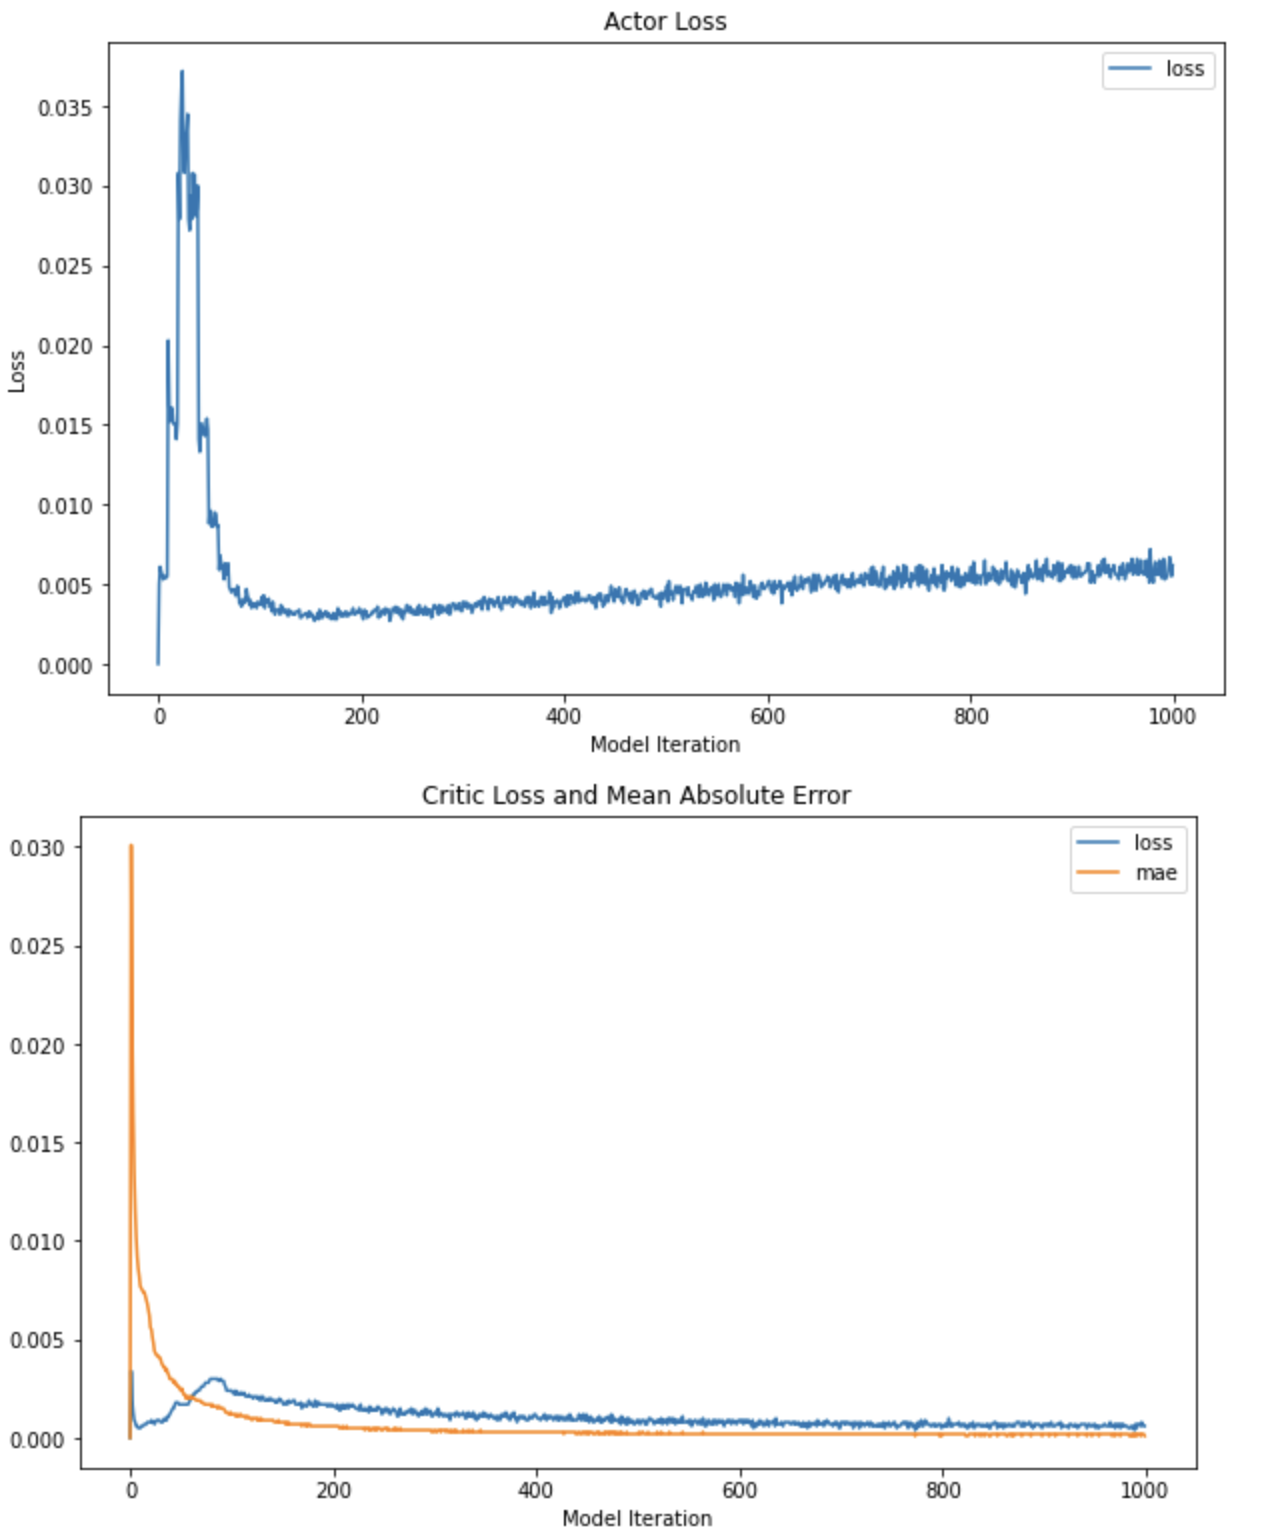
\includegraphics[width=0.47\textwidth]{ac_loss_1k.png}
    \caption{\textit{ Actor-ctiric training loss over 1000 chess games.}}
    \label{fig:ac_a_loss}
\end{figure}

\begin{figure}[!ht]
    \centering
    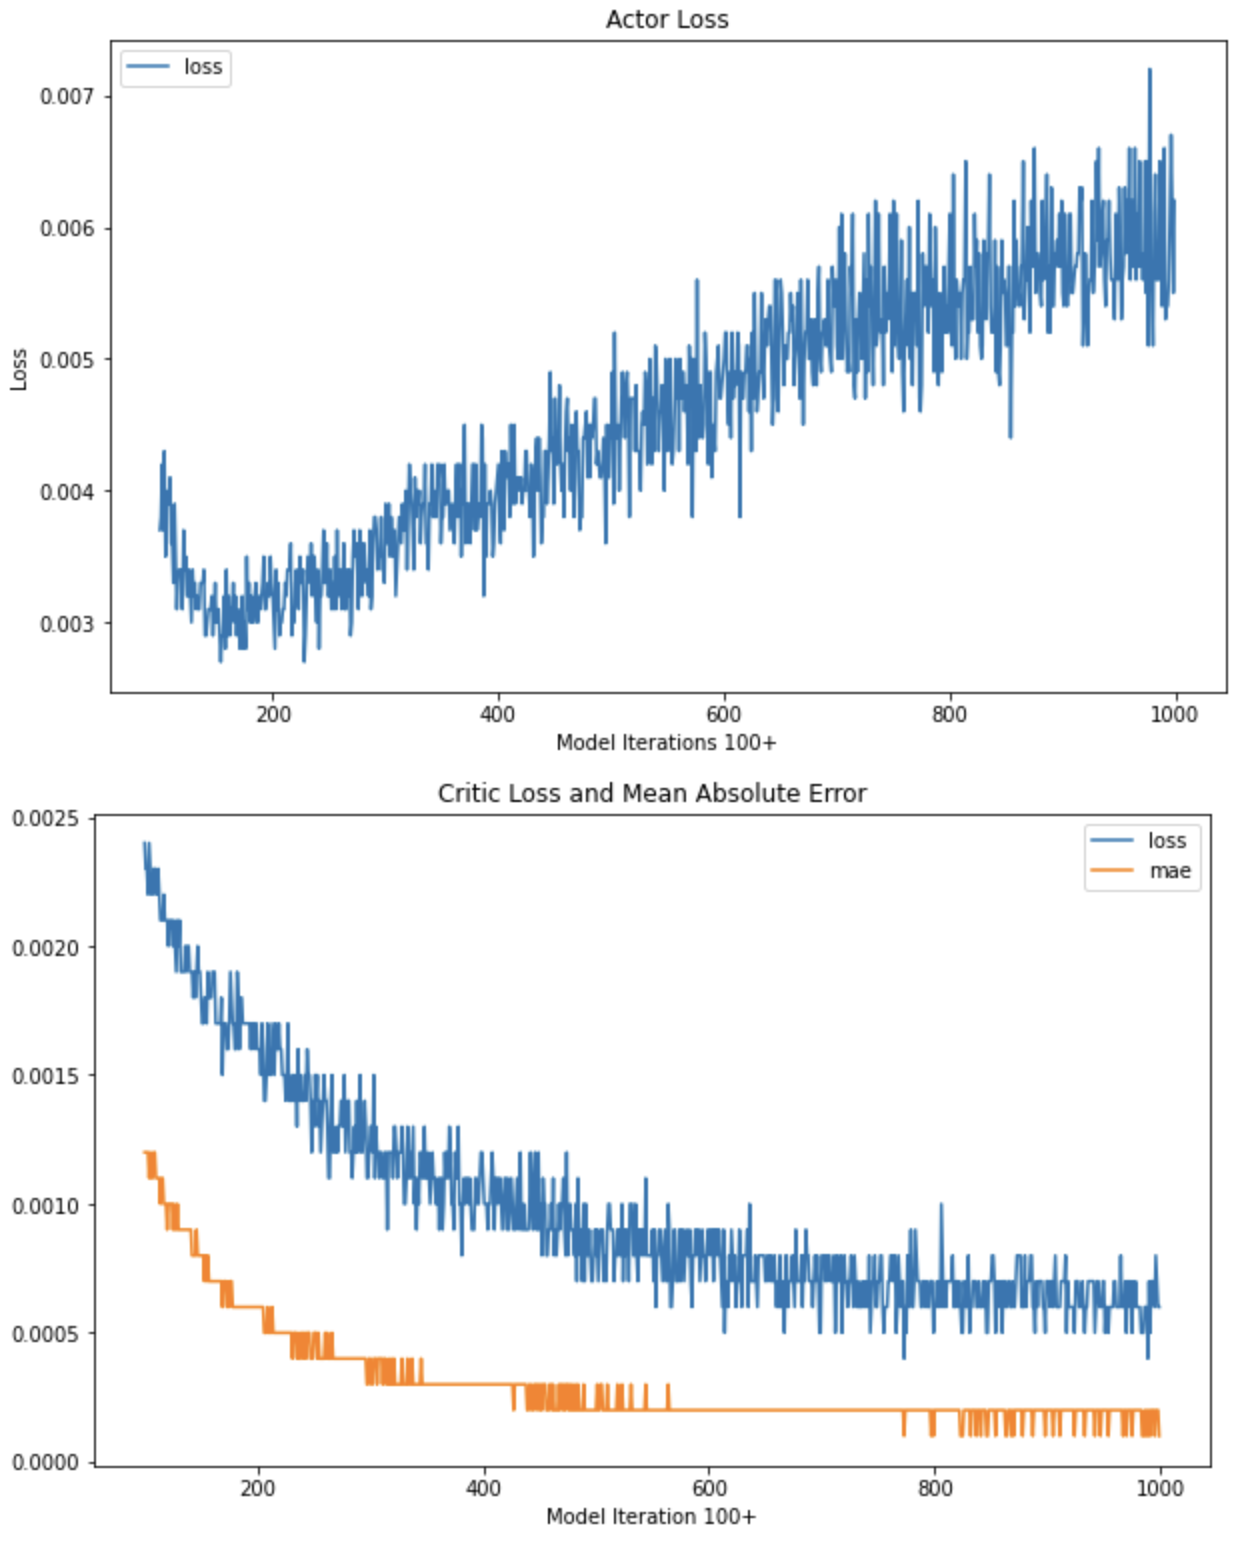
\includegraphics[width=0.47\textwidth]{ac_loss_200-1k.png}
    \caption{\textit{ Actor-ctiric training loss for games 100 to 1000.}}
    \label{fig:ac_a_loss_200}
\end{figure}

Figure \ref{fig:ac_a_loss_200} shows the actor and critic loss from episode 100 onward. We have a concern that the loss bounces around from game to game. The critic network is trending in the right direction, but training times out because we eventually exhaust the RAM in our Google Colab instances. One can argue that the loss is not meaningful since the data is purely statistical without any engineered features. A second discussion point is that the learning rate may be too large. We dismiss this argument because the overall trend in the critic’s loss is zero. The critic network can benefit from a pruned buffer that holds a good balance between wins, losses, and draws. We can also train the model on endgame examples to promote finishing games. We can also train the model for thousands more games. 

\subsection{Monte Carlo Tree Search}

We apply the Upper Confidence Bounds for Trees (UCT) algorithm to chess for our Monte Carlo Search Tree agent. We define rewards as +1 for wins, -1 for losses, and 0 for draws. During the selection portion of the algorithm, our agent uses an upper confidence bound tree policy defined as follows: 

\[A_t = \argmax_a{Q_t(a) + c \sqrt{\frac{parent visits}{visits}}} \]

Where $Q_a(t) = \frac{wins}{games + 1}$ and $c$ is the exploration hyperparameter. During the rollout, our agent follows a random action-selection policy. 10,000 iterations are performed for each move. On successive moves, the portions of the search tree are re-used when possible. Our agent plays chess against a random agent and Stockfish.

When the exploration hyperparameter $c$ is  1, the search agent explores very little. This results in the agent moving the same piece many times in a row. We had better success when increasing the parameter to 4.0. This allowed the agent to play with all pieces yet move the same piece twice when necessary. 

Due to the large branching factor in chess, we find that 10,000 iterations per move are woefully underpowered for a Monte Carlo search tree agent. This is likely due to the random rollout policy's high variance, low bias characteristics. As a result, our agent can handily beat a random agent in $\approx20$ moves. Yet, it will sometimes miss an obvious move (e.g., taking the opposing queen with a pawn). 

\section{Discussion \& Future Works}
As expected, the TDL AlphaGo Zero model achieved better performance than the standard AlphaGo Zero model with the same amount of training time, but not by as much as we expected. We note that an excessive number of games ended in ties during the training and evaluation process. For the AlphaGo Zero models, in particular, the agent would very frequently draw games due to the 75 move rule, whereby a game automatically ends in a draw if neither player moves a pawn or captures another piece for 75 moves. This notably happened frequently in situations where the agent had an overwhelming material advantage against its opponents; in other words, the agent drew games where any competent chess player should win. 

We have two ideas to address this issue in future iterations. The first is to punish draws more heavily than we currently do. For example, the reward function gave the agent one point for winning, zero points for a tie, and negative-one points for losing. The agents might learn to win more games if we gave them a penalty of negative one-half points for a draw. 

Another approach to resolving this issue draws on the observation that the agent is stalemating in positions from which it should easily win. We hypothesize that these endgame positions have not appeared frequently enough in our training data for the agent to learn an appropriate policy. Instead, these positions appear only in the endgame. We could improve performance by training the agent first on how to handle various endgame positions, still through self-play, before training it to play games from the beginning. We hypothesize that this would enable the agents to learn appropriate policies for these endgame positions that they have not explored thoroughly without overly increasing our computational requirements. 


\clearpage
\printbibliography[title={References}]
\end{document}

